\documentclass{amsart}

\title{The Dynkin diagrams package \\ Version 3.1415}

\makeatletter
\DeclareRobustCommand{\scotsMc}{\scotsMcx{c}}
\DeclareRobustCommand{\scotsMC}{\scotsMcx{\textsc{c}}}
\DeclareRobustCommand{\scotsMcx}[1]{%
  M%
  \raisebox{\dimexpr\fontcharht\font`M-\height}{%
    \check@mathfonts\fontsize{\sf@size}{0}\selectfont
    \kern.3ex\underline{\kern-.3ex #1\kern-.3ex}\kern.3ex
  }%
}
\expandafter\def\expandafter\@uclclist\expandafter{%
  \@uclclist\scotsMc\scotsMC
}
\makeatother

\author{Ben \scotsMc{}Kay}
\address{School of Mathematical Sciences,  University College Cork, Cork, Ireland}
\email{b.mckay@ucc.ie}
\date{18 December 2018}
 
\usepackage{etex}
\usepackage[T1]{fontenc}
\usepackage[utf8]{inputenx}
\usepackage{etoolbox} 
\usepackage{lmodern}
\usepackage[kerning=true,tracking=true]{microtype}
\usepackage{amsmath}
\usepackage{amsfonts}
\usepackage{array}
\usepackage{xstring}
\usepackage{longtable}
\usepackage[listings]{tcolorbox} 
\tcbuselibrary{breakable}
\tcbuselibrary{skins}
\usepackage[pdftex]{hyperref}
\hypersetup{
  colorlinks   = true,  %Colours links instead of ugly boxes
  urlcolor     = black, %Colour for external hyperlinks
  linkcolor    = black, %Colour of internal links
  citecolor    = black  %Colour of citations
}
\usepackage{booktabs}
\usepackage{colortbl}
\usepackage{varwidth}
\usepackage{dynkin-diagrams}
\usepackage{fancyvrb}
\usepackage{xspace}
\newcommand{\TikZ}{Ti\textit{k}Z\xspace}
\usepackage{filecontents}
\usetikzlibrary{decorations.markings}
\usetikzlibrary{decorations.pathmorphing}
\arrayrulecolor{white}
\makeatletter
    \def\rulecolor#1#{\CT@arc{#1}}
    \def\CT@arc#1#2{%
      \ifdim\baselineskip=\z@\noalign\fi
      {\gdef\CT@arc@{\color#1{#2}}}}
    \let\CT@arc@\relax
\rulecolor{white}
\makeatother

\newcommand{\C}[1]{\mathbb{C}^{#1}}
\renewcommand*{\arraystretch}{1.5}
\NewDocumentCommand\wdtA{}{.7cm}
\NewDocumentCommand\wdtD{}{3cm}
\NewDocumentCommand\wdtE{}{6cm}
\NewDocumentCommand\wdtL{}{3cm}
\newcolumntype{A}{@{}>{\columncolor[gray]{.9}$}m{\wdtA}<{$}} 
\newcolumntype{B}{@{}>{\columncolor[gray]{.9}}m{\wdtA}} 
\newcolumntype{D}{>{\columncolor[gray]{.9}}m{\wdtD}}
\newcolumntype{E}{>{\columncolor[gray]{.9}}m{\wdtE}}
\newcolumntype{L}{>{\columncolor[gray]{.9}}p{\wdtL}}
\newcolumntype{M}{>{\columncolor[gray]{.9}}l}
\newcolumntype{P}{>{\columncolor[gray]{.9}}p{10cm}}
\NewDocumentCommand\textleftcurly{}{\texttt{\char'173}}%
\NewDocumentCommand\textrightcurly{}{\texttt{\char'175}}%
\NewDocumentCommand\csDynkin{omom}%
{%
	\texttt{\detokenize{\dynkin}\!\!\!%
	\IfNoValueTF{#1}{}{[#1]}%
	\textleftcurly#2\textrightcurly%
	\IfNoValueTF{#3}{}{[#3]}%
	\textleftcurly#4\textrightcurly%
	}%
}%

\NewDocumentCommand\dynk{omom}%
{%
	\dynkin[#1]{#2}[#3]{#4}&\csDynkin[#1]{#2}[#3]{#4}\\
}%

\NewDocumentCommand\typesetSubseries{m}%
{%
	\IfInteger{#1}{#1}{\IfStrEq{#1}{}{n}{#1}}
}%

\NewDocumentCommand\dyn{omom}%
{%
	{#2}_{\typesetSubseries{#4}}^{\IfInteger{#3}{#3}{\IfStrEq{#1}{extended}{1}{}}} & \dynk[#1]{#2}[#3]{#4}%
}%


\NewDocumentEnvironment{dynkinTable}{mmm}%
{%
\RenewDocumentCommand\wdtD{}{#2}
\RenewDocumentCommand\wdtL{}{#3}
\begin{longtable}{ADM}
\caption{#1}\\
\endfirsthead
\caption{\dots continued}\\
\endhead
\multicolumn{2}{c}{continued \dots}\\
\endfoot
\endlastfoot
}%
{%
\end{longtable}
}%


\definecolor{example-color}{gray}{.85}
\definecolor{example-border-color}{gray}{.7} 

\tcbset{coltitle=black,colback=example-color,colframe=example-border-color,enhanced,breakable,pad at break*=1mm,
toprule=1.2mm,bottomrule=1.2mm,leftrule=1mm,rightrule=1mm,toprule at break=-1mm,bottomrule at break=-1mm,
before upper={\widowpenalties=3 10000 10000 150}}

\makeatletter
\def\@tocline#1#2#3#4#5#6#7{\relax
  \ifnum #1>\c@tocdepth%
  \else
    \par \addpenalty\@secpenalty\addvspace{#2}%
    \begingroup \hyphenpenalty\@M
    \@ifempty{#4}{%
      \@tempdima\csname r@tocindent\number#1\endcsname\relax
    }{%
      \@tempdima#4\relax
    }%
    \parindent\z@ \leftskip#3\relax \advance\leftskip\@tempdima\relax
    #5\leavevmode\hskip-\@tempdima #6\nobreak\relax
    ,~#7\par
    \endgroup
  \fi}
\makeatother

\fvset{fontsize=\small}

\begin{document}

\maketitle
\begin{center}
\begin{varwidth}{\textwidth}
\tableofcontents
\end{varwidth}
\end{center}


\setlength{\arrayrulewidth}{1.5pt}

\section{Quick introduction}
\begin{tcolorbox}[title={Load the Dynkin diagram package (see options below)}]
\begin{verbatim}
\documentclass{amsart}
\usepackage{dynkin-diagrams} 
\begin{document}
The Dynkin diagram of \(B_3\) is \dynkin{B}{3}.
\end{document}
\end{verbatim}
\end{tcolorbox}
\begin{tcblisting}{title={Invoke it}}
The Dynkin diagram of \(B_3\) is \dynkin{B}{3}.
\end{tcblisting}
\begin{tcblisting}{title={Inside a \TikZ statement}}
The Dynkin diagram of \(B_3\) is 
\tikz \dynkin{B}{3};
\end{tcblisting}
\begin{tcblisting}{title={Inside a Dynkin diagram environment}}
The Dynkin diagram of \(B_3\) is 
\begin{dynkinDiagram}{B}{3}
\draw[very thick,red] (root 1) to [out=-45, in=-135] (root 3);
\end{dynkinDiagram}
\end{tcblisting}
\begin{tcblisting}{title={Inside a \TikZ environment}}
The baseline controls the vertical alignment:
the Dynkin diagram of \(B_3\) is 
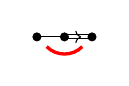
\begin{tikzpicture}[baseline=(origin.base)]
\dynkin{B}{3}
\draw[very thick,red] (root 1) to [out=-45, in=-135] (root 3);
\end{tikzpicture}
\end{tcblisting}
\begin{tcblisting}{title={Indefinite rank Dynkin diagrams}}
\dynkin{B}{}
\end{tcblisting}

\begin{dynkinTable}{The Dynkin diagrams of the reduced simple root systems \cite{Bourbaki:2002} pp. 265--290, plates I--IX}{2.25cm}{2.5cm}
\dyn{A}{}
\dyn{C}{}
\dyn{D}{}
\dyn{E}{6}
\dyn{E}{7}
\dyn{E}{8}
\dyn{F}{4}
\dyn{G}{2}
\end{dynkinTable}


\section{Set options globally}

\begin{tcolorbox}[title={Most options set globally \dots}]
\begin{verbatim}
\pgfkeys{/Dynkin diagram,edge length=.5cm,fold radius=.5cm,
indefinite edge/.style={
    draw=black,fill=white,thin,densely dashed}}
\end{verbatim}
\end{tcolorbox}
You can also pass options to the package in \verb!\usepackage!.
\emph{Danger:} spaces in option names are replaced with hyphens: \texttt{edge length=1cm} is \texttt{edge-length=1cm} as a global option; moreover you should drop the extension \verb!/.style! on any option with spaces in its name (but not otherwise). For example,
\begin{tcolorbox}[title={\dots or pass global options to the package}]
\begin{verbatim}
\usepackage[
     ordering=Kac,
     edge/.style=blue,
	indefinite-edge={draw=green,fill=white,densely dashed},
	indefinite-edge-ratio=5,
     mark=o,
     root-radius=.06cm]
     {dynkin-diagrams}
\end{verbatim}
\end{tcolorbox}



\section{Coxeter diagrams}

\begin{tcblisting}{title={Coxeter diagram option}}
\dynkin[Coxeter]{F}{4}
\end{tcblisting}

\begin{tcblisting}{title={gonality option for \(G_2\) and \(I_n\) Coxeter diagrams}}
\(G_2=\dynkin[Coxeter,gonality=n]{G}{2}\), \ 
\(I_n=\dynkin[Coxeter,gonality=n]{I}{}\)
\end{tcblisting}

\begin{dynkinTable}{The Coxeter diagrams of the simple reflection groups}{2.25cm}{6cm}
\dyn[Coxeter]{A}{}
\dyn[Coxeter]{B}{}
\dyn[Coxeter]{C}{}
\dyn[Coxeter]{E}{6}
\dyn[Coxeter]{E}{7}
\dyn[Coxeter]{E}{8}
\dyn[Coxeter]{F}{4}
\dyn[Coxeter,gonality=n]{G}{2}
\dyn[Coxeter]{H}{3}
\dyn[Coxeter]{H}{4}
\dyn[Coxeter,gonality=n]{I}{}
\end{dynkinTable}

\section{Satake diagrams}\label{section:Satake}

\begin{tcblisting}{title={Satake diagrams use the standard name instead of a rank}}
\(A_{IIIb}=\dynkin{A}{IIIb}\)
\end{tcblisting}

We use a solid gray bar to denote the folding of a Dynkin diagram, rather than the usual double arrow, since the diagrams turn out simpler and easier to read.

\begin{dynkinTable}{The Satake diagrams of the real simple Lie algebras \cite{Helgason:2001} p. 532--534}{2.75cm}{3cm}
\dyn{A}{I}
\dyn{A}{II}
\dyn{A}{IIIa}
\dyn{A}{IIIb}
\dyn{A}{IV}
\dyn{B}{I}
\dyn{B}{II}
\dyn{C}{I}
\dyn{C}{IIa}
\dyn{C}{IIb}
\dyn{D}{Ia}
\dyn{D}{Ib}
\dyn{D}{Ic}
\dyn{D}{II}
\dyn{D}{IIIa}
\dyn{D}{IIIb}
\dyn{E}{I}
\dyn{E}{II}
\dyn{E}{III}
\dyn{E}{IV}
\dyn{E}{V}
\dyn{E}{VI}
\dyn{E}{VII}
\dyn{E}{VIII}
\dyn{E}{IX}
\dyn{F}{I}
\dyn{F}{II}
\dyn{G}{I}
\end{dynkinTable}

\begin{tcblisting}{title={If you don't like the solid gray ``folding bar'', most people use arrows. Here is \(E_{II}\)}}
\newcommand{\invol}[2]{\draw[latex-latex] (root #1) to 
[out=-60,in=-120] node[midway,below]{$\sigma$} (root #2);}
\begin{dynkinDiagram}[edge length=.75cm,labels*={1,...,6}]{E}{6}
\invol{1}{6}\invol{3}{5}
\end{dynkinDiagram}
\end{tcblisting}

\begin{tcblisting}{title={The double arrows for \(A_{IIIa}\) are big}}
\newcommand{\invol}[2]{\draw[latex-latex] (root #1) to 
[out=-60,in=-120] node[midway,below]{$\sigma$} (root #2);}
\begin{dynkinDiagram}[edge length=.75cm]{A}{oo.o**.**o.oo}
\invol{1}{10}\invol{2}{9}\invol{3}{8}\invol{4}{7}\invol{5}{6}
\end{dynkinDiagram}
\end{tcblisting}

\begin{tcblisting}{title={If you don't like the solid gray ``folding bar'', most people use arrows \dots}}
\tikzset{/Dynkin diagram/fold style/.style={stealth-stealth,thick,
shorten <=1mm,shorten >=1mm,}}
\dynkin[ply=3,edge length=.75cm]{D}{4}
\begin{dynkinDiagram}[ply=4]{D}[1]%
{****.*****.*****}
	\dynkinFold{1}{13}
	\dynkinFold[bend right=65]{0}{14}
\end{dynkinDiagram}
\end{tcblisting}

\begin{tcblisting}{title={\dots but you could try springs pulling roots together}}
\tikzset{/Dynkin diagram/fold style/.style=
{decorate,decoration={name=coil,aspect=0.5,
segment length=1mm,amplitude=.6mm}}}
\dynkin[ply=3,edge length=.75cm]{D}{4}
\begin{dynkinDiagram}[ply=4]{D}[1]%
{****.*****.*****}
	\dynkinFold{1}{13}
	\dynkinFold[bend right=65]{0}{14}
\end{dynkinDiagram}
\end{tcblisting}


\section{Labels for the roots}

\begin{tcblisting}{title={Make a macro to assign labels to roots}}
\dynkin[label,label macro/.code={\alpha_{#1}},edge length=.75cm]{D}{5}
\end{tcblisting}
\begin{tcblisting}{title={Labelling several roots}}
\dynkin[labels={,2,...,5,,7},label macro/.code={\alpha_{#1}}]{A}{7}
\end{tcblisting}
\begin{tcblisting}{title={The \texttt{foreach} notation I}}
\dynkin[labels={1,3,...,7},]{A}{9}
\end{tcblisting}
\begin{tcblisting}{title={The \texttt{foreach} notation II}}
\dynkin[labels={,\alpha_2,\alpha_...,\alpha_7},]{A}{7}
\end{tcblisting}
\begin{tcblisting}{title={The \texttt{foreach} notation III}}
\dynkin[label macro/.code={\beta_{#1}},labels={,2,...,7},]{A}{7}
\end{tcblisting}
\begin{tcblisting}{title={Label the roots individually by root number}}
\dynkin[label]{B}{3}
\end{tcblisting}
\begin{tcblisting}{title={Label a single root}}
\begin{dynkinDiagram}{B}{3}
\dynkinLabelRoot{2}{\alpha_2}
\end{dynkinDiagram}
\end{tcblisting}
\begin{tcblisting}{title={Use a text style}}
\begin{dynkinDiagram}[text/.style={scale=1.2}]{B}{3};
\dynkinLabelRoot{2}{\alpha_2}
\end{dynkinDiagram}
\end{tcblisting}
\begin{tcblisting}{title={Access root labels via TikZ}}
\begin{dynkinDiagram}{B}{3}
\node[below] at (root 2) {\(\alpha_2\)};
\end{dynkinDiagram}
\end{tcblisting}
\begin{tcblisting}{title={Commands to label several roots}}
\begin{dynkinDiagram}{A}{7} 
\dynkinLabelRoots{,\alpha_2,\alpha_3,\alpha_4,\alpha_5,,\alpha_7}
\end{dynkinDiagram}
\end{tcblisting}
\begin{tcblisting}{title={The labels have default locations, mostly below roots}}
\dynkin[edge length=.75cm,labels={1,2,3}]{E}{8}
\end{tcblisting}
\begin{tcblisting}{title={The starred form flips labels to alternate locations, mostly above roots}}
\dynkin[edge length=.75cm,labels*={1,2,3}]{E}{8}
\end{tcblisting}
\begin{tcblisting}{title={Labelling several roots and alternates}}
\dynkin[%
label macro/.code={\alpha_{#1}},
label macro*/.code={\gamma_{#1}},
labels={,2,...,5,,7},
labels*={1,3,4,5,6}]{A}{7}
\end{tcblisting}
\begin{tcblisting}{title={Commands to label several roots}}
\begin{dynkinDiagram}{A}{7} 
\dynkinLabelRoots{,\alpha_2,\alpha_3,\alpha_4,\alpha_5,,\alpha_7}
\dynkinLabelRoots*{a,b,c,d,e,f,g}
\end{dynkinDiagram}
\end{tcblisting}


\section{Bracing roots}
\begin{tcblisting}{title={Bracing roots}}
\begin{dynkinDiagram}{A}{*.*x*.*} 
\dynkinBrace[p]{1}{2}
\dynkinBrace[q]{4}{5}
\end{dynkinDiagram}
\end{tcblisting}
\begin{tcblisting}{title={Bracing roots, and a starred form}}
\begin{dynkinDiagram}{A}{10}
\dynkinBrace[\text{Roots 2 to 9}]{2}{9}
\dynkinBrace*[\text{Roots 3 to 8}]{3}{8}
\end{dynkinDiagram}
\end{tcblisting}
\begin{tcblisting}{title={Bracing roots}}
\newcommand\circleRoot[1]{\draw (root #1) circle (3pt);}
\begin{dynkinDiagram}{A}{**.***.***.***.***.**}
\circleRoot{4}\circleRoot{7}\circleRoot{10}\circleRoot{13}
\dynkinBrace[y-1]{1}{3}
\dynkinBrace[z-1]{5}{6}
\dynkinBrace[t-1]{11}{12}
\dynkinBrace[x-1]{14}{16}
\end{dynkinDiagram}
\end{tcblisting}

\begin{filecontents*}{EulerProducts.tex}
\tikzset{/Dynkin diagram,ordering=Dynkin,label macro/.code={\alpha_{#1}}}
\newcounter{EPNo}
\setcounter{EPNo}{0}
\NewDocumentCommand\EP{smmmm}%
{%
\stepcounter{EPNo}\roman{EPNo}. &
\def\eL{.6cm}
\IfStrEqCase{#2}%
{%
{D}{\gdef\eL{1cm}}%
{E}{\gdef\eL{.75cm}}%
{F}{\gdef\eL{.35cm}}%
{G}{\gdef\eL{.35cm}}%
}%
\tikzset{/Dynkin diagram,edge length=\eL}
\IfBooleanTF{#1}%
{\dynkin[backwards,labels*={#4},labels={#5}]{#2}{#3}}
{\dynkin[labels*={#4},labels={#5}]{#2}{#3}}
\\
}%
\begin{longtable}{MM}
\caption{Dynkin diagrams from Euler products \cite{Langlands:1967}}\\
\endfirsthead
\caption{\dots continued}\\
\endhead
\multicolumn{2}{c}{continued \dots}\\
\endfoot
\endlastfoot
\EP{A}{***.**}{1,1,1,1,1}{,1,2,n-1,n}
\EP{A}{***.**}{1,1,1,1,1}{1,2,n-1,n}
\EP{A}{**.***.*}{1,1,1,1,1,1}{1,2,m-1,,m,n}
\EP{B}{**.***}{2,2,2,2,1}{1,2,n-1,n}
\EP*{B}{***.**}{2,2,2,2,1}{n,n-1,2,1,}
\EP{C}{**.***}{1,1,1,1,2}{1,2,n-1,}
\EP*{C}{***.**}{1,1,1,1,2}{n,n-1,2,1,}
\EP{D}{**.****}{1,1,1,1,1,1}{1,2,n-2,n-1,n}
\EP{D}{**.****}{1,1,1,1,1,1}{1,2,n-2,n-1,n}
\EP{E}{6}{1,1,1,1,1,1}{1,...,5}
\EP*{E}{7}{1,1,1,1,1,1,1}{6,...,1}
\EP{E}{7}{1,1,1,1,1,1,1}{1,...,6}
\EP*{E}{8}{1,1,1,1,1,1,1,1}{7,...,1}
\EP{E}{8}{1,1,1,1,1,1,1,1}{1,...,7}
\EP{G}{2}{1,3}{,1}
\EP{G}{2}{1,3}{1}
\EP{B}{**.*.**}{2,2,2,2,1}{,1,2,n-1,n}
\EP{F}{4}{1,1,2,2}{,3,2,1}
\EP{C}{3}{1,1,2}{,2,1}
\EP{C}{**.***}{1,1,1,1,2}{,1,n-2,n-1,n}
\EP*{B}{3}{2,2,1}{1,2}
\EP{F}{4}{1,1,2,2}{1,2,3}
\EP{D}{**.****}{1,1,1,1,1,1}{1,2,n-2,n-2,n,n}
\EP{E}{6}{1,1,1,1,1,1}{1,2,3,4,,5}
\EP{E}{6}{1,1,1,1,1,1}{1,2,3,5,,4}
\EP*{E}{7}{1,1,1,1,1,1,1}{,5,...,1,6}
\EP*{E}{7}{1,1,1,1,1,1,1}{,6,4,3,2,1,5}
\EP*{E}{8}{1,1,1,1,1,1,1,1}{,6,...,1,7}
\EP*{E}{8}{1,1,1,1,1,1,1,1}{,7,5,4,3,2,1,6}
\EP*{E}{7}{1,1,1,1,1,1,1}{5,...,1,,6}
\EP*{E}{7}{1,1,1,1,1,1,1}{1,...,5,,6}
\EP*{E}{8}{1,1,1,1,1,1,1,1}{6,...,1,,7}
\end{longtable}
\end{filecontents*}
{\input{EulerProducts}}\VerbatimInput{EulerProducts.tex}

\section{Style}
\begin{tcblisting}{title={Colours}}
\dynkin[
	edge/.style={blue!50,thick},
	*/.style=blue!50!red,
	arrow color=red]{F}{4}
\end{tcblisting}
\begin{tcblisting}{title={Edge lengths}}
The Dynkin diagram of \(A_3\) is \dynkin[edge length=1.2,parabolic=3]{A}{3}
\end{tcblisting}
\begin{tcblisting}{title={Root marks}}
\dynkin{E}{8}
\dynkin[mark=*]{E}{8}
\dynkin[mark=o]{E}{8}
\dynkin[mark=O]{E}{8}
\dynkin[mark=t]{E}{8}
\dynkin[mark=x]{E}{8}
\dynkin[mark=X]{E}{8}
\end{tcblisting}
At the moment, you can only use:
\par\noindent\begin{tabular}{>{\ttfamily}cl}
* & solid dot \\
o & hollow circle \\
O & double hollow circle \\
t & tensor root \\
x & crossed root \\ 
X & thickly crossed root 
\end{tabular}
\begin{tcblisting}{title={Mark styles}}
The parabolic subgroup \(E_{8,124}\) is \dynkin[parabolic=124,x/.style={brown,very thick}]{E}{8}
\end{tcblisting}
\begin{tcblisting}{title={Sizes of root marks}}
\(A_{3,3}\) with big root marks is \dynkin[root radius=.08cm,parabolic=3]{A}{3}
\end{tcblisting}


\section{Suppress or reverse arrows}
\begin{tcblisting}{title={Some diagrams have double or triple edges}}
\dynkin{F}{4}
\dynkin{G}{2}
\end{tcblisting}
\begin{tcblisting}{title={Suppress arrows}}
\dynkin[arrows=false]{F}{4}
\dynkin[arrows=false]{G}{2}
\end{tcblisting}
\begin{tcblisting}{title={Reverse arrows}}
\dynkin[reverse arrows]{F}{4}
\dynkin[reverse arrows]{G}{2}
\end{tcblisting}


\section{Backwards and upside down}

\begin{tcblisting}{title={Default}}
\dynkin{E}{8}
\dynkin{F}{4}
\dynkin{G}{2}
\end{tcblisting}
\begin{tcblisting}{title={Backwards}}
\dynkin[backwards]{E}{8}
\dynkin[backwards]{F}{4}
\dynkin[backwards]{G}{2}
\end{tcblisting}
\begin{tcblisting}{title={Reverse arrows}}
\dynkin[reverse arrows]{F}{4}
\dynkin[reverse arrows]{G}{2}
\end{tcblisting}
\begin{tcblisting}{title={Backwards, reverse arrows}}
\dynkin[backwards,reverse arrows]{F}{4}
\dynkin[backwards,reverse arrows]{G}{2}
\end{tcblisting}
\begin{tcblisting}{title={Backwards versus upside down}}
\dynkin[label]{E}{8}
\dynkin[label,backwards]{E}{8}
\dynkin[label,upside down]{E}{8}
\dynkin[label,backwards,upside down]{E}{8}
\end{tcblisting}


\section{Drawing on top of a Dynkin diagram}

\begin{tcblisting}{title={TikZ can access the roots themselves}}
\begin{dynkinDiagram}{A}{4}
	\fill[white,draw=black] (root 2) circle (.15cm);
	\fill[white,draw=black] (root 2) circle (.1cm);
	\draw[black] (root 2) circle (.05cm);
\end{dynkinDiagram}
\end{tcblisting}
\begin{tcblisting}{title={Draw curves between the roots}}
\begin{dynkinDiagram}[label]{E}{8}
	\draw[very thick, black!50,-latex]  
		(root 3.south) to [out=-45, in=-135] (root 6.south); 
\end{dynkinDiagram}
\end{tcblisting}
\begin{tcblisting}{title={Change marks}}
\begin{dynkinDiagram}[mark=o,label]{E}{8}
	\dynkinRootMark{*}{5}
	\dynkinRootMark{*}{8}
\end{dynkinDiagram}
\end{tcblisting}


\section{Mark lists}

The package allows a list of root marks instead of a rank:

\begin{tcblisting}{title={A mark list}}
\dynkin{E}{oo**ttxx}
\end{tcblisting}
The mark list \verb!oo**ttxx! has one mark for each root: \verb!o!, \verb!o!, \dots, \verb!x!.
Roots are listed in the current default ordering.
(Careful: in an affine root system, a mark list will \emph{not} contain a mark for root zero.)

If you need to repeat a mark, you can give a \emph{single digit} positive integer to indicate how many times to repeat it.
\begin{tcblisting}{title={A mark list with repetitions}}
\dynkin{A}{x4o3t4}
\end{tcblisting}

\NewDocumentCommand\ClassicalLieSuperalgebras{om}%
{%
\IfValueT{#1}{\tikzset{/Dynkin diagram,root radius=#1}}
\RenewDocumentCommand\wdtE{}{10cm}
\begin{dynkinTable}{Classical Lie superalgebras \cite{Frappat/Sciarrino/Sorba:1989}. #2}{3.5cm}{6.5cm}
\IfValueT{#1}{
& & \texttt{\textbackslash{}tikzset\{/Dynkin diagram,root radius=#1\}} \\
}
A_{mn} & \dynk{A}{o3.oto.oo}
B_{mn} & \dynk{B}{o3.oto.oo}
B_{0n} & \dynk{B}{o3.o3.o*}
C_{n}  & \dynk{C}{too.oto.oo}
D_{mn} & \dynk{D}{o3.oto.o4}
D_{21\alpha} & \dynk{A}{oto}
F_4 & \dynk{F}{ooot}
G_3 & \dynk[extended,affine mark=t,
reverse arrows]{G}{2} 
\end{dynkinTable}
\IfValueT{#1}{\tikzset{/Dynkin diagram,root radius=.05cm}}
}%

\ClassicalLieSuperalgebras[.07cm]{We need a slightly larger root radius parameter to distinguish the tensor product symbols from the solid dots.}

\ClassicalLieSuperalgebras{Here we see the problem with using the default root radius parameter, which is too small for tensor product symbols.}



\section{Indefinite edges}

An \emph{indefinite edge} is a dashed edge between two roots, \dynkin{A}{*.*} indicating that an indefinite number of roots have been omitted from the Dynkin diagram.
In between any two entries in a mark list, place a period to indicate an indefinite edge:
\begin{tcblisting}{title={Indefinite edges}}
\dynkin{D}{o.o*.*.t.to.t}
\end{tcblisting}

In certain diagrams, roots may have an edge between them even though they are not subsequent in the ordering.
For such rare situations, there is an option:
\begin{tcblisting}{title={Indefinite edge option}}
\dynkin[make indefinite edge={3-5},label]{D}{5}
\end{tcblisting}
\begin{tcblisting}{title={Give a list of edges to become indefinite}}
\dynkin[make indefinite edge/.list={1-2,3-5},label]{D}{5}
\end{tcblisting}

\begin{tcblisting}{title={Indefinite edge style}}
\dynkin[indefinite edge/.style={draw=black,fill=white,thin,densely dashed},%
	edge length=1cm,%
	make indefinite edge={3-5}]
	{D}{5}
\end{tcblisting}

\begin{tcblisting}{title={The ratio of the lengths of indefinite edges to those of other edges}}
\dynkin[edge length = .5cm,%
	indefinite edge ratio=3,%
	make indefinite edge={3-5}]
	{D}{5}
\end{tcblisting}


\begingroup
\RenewDocumentCommand\wdtA{}{.35cm}
\RenewDocumentCommand\wdtE{}{6.55cm}
\begin{dynkinTable}{Springer's table of indices \cite{Springer:2009}, pp. 320-321, with one form of \(E_7\) corrected}{2.5cm}{3.7cm}
% 1
A_n &
\multicolumn{2}{E}{
\begin{dynkinDiagram}{A}{o.o*o.o*o.o}
\dynkinLabelRoot{3}{d}
\dynkinLabelRoot{6}{n-d}
\end{dynkinDiagram}
}
\\
% 2
A_n &
\multicolumn{2}{E}{
\begin{dynkinDiagram}{A}{o.o*o.o*o.o*o.o*o.o}
\dynkinLabelRoot{3}{d}
\dynkinLabelRoot{6}{rd}
\dynkinLabelRoot{9}{n-rd}
\dynkinLabelRoot{12}{n-d}
\end{dynkinDiagram}
}
\\
% 3
B_n &
\multicolumn{2}{E}{
\begin{dynkinDiagram}{B}{**.*.o.oo}
\dynkinLabelRoot{3}{r}
\end{dynkinDiagram}
}
\\
% 4
C_n &
\multicolumn{2}{E}{
\begin{dynkinDiagram}{C}{o.o*o.o*o.oo}
\dynkinLabelRoot{3}{d}
\dynkinLabelRoot{6}{rd}
\end{dynkinDiagram}
}
\\
% 5
D_n &
\multicolumn{2}{E}{
\begin{dynkinDiagram}{D}{o.o*o.o*o.ooo}
\dynkinLabelRoot{3}{d}
\dynkinLabelRoot{6}{rd}
\end{dynkinDiagram}
}
\\
% 6
E_6 &
\dynk{E}{*oooo*}
% 7
E_6 &
\dynk{E}{o*o*oo}
% 8
E_6 &
\dynk{E}{o*oooo}
% 9
E_6 &
\dynk{E}{**ooo*}
% 10
E_7 &
\dynk{E}{*oooooo}
% 11
E_7 &
\dynk{E}{ooooo*o}
% 12
E_7 &
\dynk{E}{oooooo*}
% 13
E_7 &
\dynk{E}{*oooo*o}
% 14 - corrected from Springer.
E_7 &
\dynk{E}{*oooo**}
% 15
E_7 &
\dynk{E}{*o**o*o}
% 16
E_8 &
\dynk{E}{*ooooooo}
% 17
E_8 &
\dynk{E}{ooooooo*}
% 18
E_8 &
\dynk{E}{*oooooo*}
% 19
E_8 &
\dynk{E}{oooooo**}
% 20
E_8 &
\dynk{E}{*oooo***}
% 21
F_4 &
\dynk{F}{ooo*}
% 22
D_4 & 
\dynk{D}{o*oo}
\end{longtable}
\endgroup




\section{Parabolic subgroups}

Each set of roots is assigned a number, with each binary digit zero or one to say whether the corresponding root is crossed or not:
\begin{tcblisting}{}
The flag variety of pointed lines in 
projective 3-space is associated to 
the Dynkin diagram \dynkin[parabolic=3]{A}{3}.
\end{tcblisting}

\begin{filecontents*}{hermitian-symmetric-spaces.tex}
\NewDocumentCommand\HSS{mommm}
{#1&\IfNoValueTF{#2}{\dynkin{#3}{#4}}{\dynkin[parabolic=#2]{#3}{#4}}&#5\\}
\renewcommand*{\arraystretch}{1.5}
\begin{longtable}
{>{\columncolor[gray]{.9}}>$l<$>{\columncolor[gray]{.9}}>$l<$>{\columncolor[gray]{.9}}l}
\caption{The Hermitian symmetric spaces}\endfirsthead
\caption{\dots continued}\\ \endhead
\caption{continued \dots}\\ \endfoot
\endlastfoot
\HSS{A_n}{A}{**.*x*.**}{Grassmannian of $k$-planes in $\C{n+1}$}
\HSS{B_n}[1]{B}{}{$(2n-1)$-dimensional hyperquadric, i.e. the variety of null lines in $\C{2n+1}$}
\HSS{C_n}[16]{C}{}{space of Lagrangian $n$-planes in $\C{2n}$}
\HSS{D_n}[1]{D}{}{$(2n-2)$-dimensional hyperquadric, i.e. the variety of null lines in $\C{2n}$}
\HSS{D_n}[32]{D}{}{one component of the variety of maximal dimension null subspaces of $\C{2n}$}
\HSS{D_n}[16]{D}{}{the other component}
\HSS{E_6}[1]{E}{6}{complexified octave projective plane}
\HSS{E_6}[32]{E}{6}{its dual plane}
\HSS{E_7}[64]{E}{7}{the space of null octave 3-planes in octave 6-space}
\end{longtable}
\end{filecontents*}
\begingroup
\input{hermitian-symmetric-spaces.tex}
\endgroup
\VerbatimInput{hermitian-symmetric-spaces.tex}

\begin{tcblisting}{title={Folded parabolics look bad (zoom in on a root)}}
\dynkin[fold,parabolic=3]{C}{2}
\dynkin[fold,parabolic=3]{G}{2}
\end{tcblisting}
\begin{tcblisting}{title={Folded parabolics: you can try using thicker crosses}}
\dynkin[fold,x/.style={very thick,line cap=round},parabolic=3]{C}{2}
\dynkin[fold,x/.style={ultra thick,line cap=round},parabolic=3]{G}{2}
\end{tcblisting}


\section{Extended Dynkin diagrams}

\begin{tcblisting}{title={Extended Dynkin diagrams}}
\dynkin[extended]{A}{7}
\end{tcblisting}


The extended Dynkin diagrams are also described in the notation of Kac \cite{Kac:1990} p. 55 as affine untwisted Dynkin diagrams: we extend \verb!\dynkin{A}{7}! to become \verb!\dynkin{A}[1]{7}!:
\begin{tcblisting}{title={Extended Dynkin diagrams}}
\dynkin{A}[1]{7}
\end{tcblisting}


\renewcommand*{\arraystretch}{1.5}
\begin{dynkinTable}{The Dynkin diagrams of the extended simple root systems}{3cm}{5cm}
\dyn[extended]{A}{1}
\dyn[extended]{A}{}
\dyn[extended]{B}{}
\dyn[extended]{C}{}
\dyn[extended]{D}{}
\dyn[extended]{E}{6}
\dyn[extended]{E}{7}
\dyn[extended]{E}{8}
\dyn[extended]{F}{4}
\dyn[extended]{G}{2}
\end{dynkinTable}





\section{Affine twisted and untwisted Dynkin diagrams}

The affine Dynkin diagrams are described in the notation of Kac \cite{Kac:1990} p. 55:
\begin{tcblisting}{title={Affine Dynkin diagrams}}
\(A^{(1)}_7=\dynkin{A}[1]{7}, \ 
E^{(2)}_6=\dynkin{E}[2]{6}, \ 
D^{(3)}_4=\dynkin{D}[3]{4}\)
\end{tcblisting}



\begin{dynkinTable}{The affine Dynkin diagrams}{3cm}{3.75cm}
\dyn{A}[1]{1}
\dyn{A}[1]{}
\dyn{B}[1]{}
\dyn{C}[1]{}
\dyn{D}[1]{}
\dyn{E}[1]{6}
\dyn{E}[1]{7}
\dyn{E}[1]{8}
\dyn{F}[1]{4}
\dyn{G}[1]{2}
\dyn{A}[2]{2}
\dyn{A}[2]{even}
\dyn{A}[2]{odd}
\dyn{D}[2]{}
\dyn{E}[2]{6}
\dyn{D}[3]{4}
\end{dynkinTable}

\begin{dynkinTable}{Some more affine Dynkin diagrams}{3cm}{3.25cm}
\dyn{A}[2]{4}
\dyn{A}[2]{5}
\dyn{A}[2]{6}
\dyn{A}[2]{7}
\dyn{A}[2]{8}
\dyn{D}[2]{3}
\dyn{D}[2]{4}
\dyn{D}[2]{5}
\dyn{D}[2]{6}
\dyn{D}[2]{7}
\dyn{D}[2]{8}
\dyn{D}[3]{4}
\dyn{E}[2]{6}
\end{dynkinTable}




\section{Extended Coxeter diagrams}

\begin{tcblisting}{title={Extended and Coxeter options together}}
\dynkin[extended,Coxeter]{F}{4}
\end{tcblisting}


\begin{dynkinTable}{The extended (affine) Coxeter diagrams}{3cm}{6cm}
\dyn[extended,Coxeter]{A}{}
\dyn[extended,Coxeter]{B}{}
\dyn[extended,Coxeter]{C}{}
\dyn[extended,Coxeter]{D}{}
\dyn[extended,Coxeter]{E}{6}
\dyn[extended,Coxeter]{E}{7}
\dyn[extended,Coxeter]{E}{8}
\dyn[extended,Coxeter]{F}{4}
\dyn[extended,Coxeter]{G}{2}
\dyn[extended,Coxeter]{H}{3}
\dyn[extended,Coxeter]{H}{4}
\dyn[extended,Coxeter]{I}{1}
\end{dynkinTable}

\section{Kac style}
We include a style called \verb!Kac! which tries to imitate the style of \cite{Kac:1990}.
\begin{tcblisting}{title={Kac style}}
\dynkin[Kac]{F}{4}
\end{tcblisting}
\begingroup
\pgfkeys{/Dynkin diagram,Kac}
\begin{dynkinTable}{The Dynkin diagrams of the simple root systems in Kac style}{5cm}{4.5cm}
\dyn{A}{}
\dyn{B}{}
\dyn{C}{}
\dyn{D}{}
\dyn{E}{6}
\dyn{E}{7}
\dyn{E}{8}
\dyn{F}{4}
\dyn{G}{2}
\end{dynkinTable}
\begin{dynkinTable}{The Dynkin diagrams of the extended simple root systems in Kac style}{5cm}{4.5cm}
\dyn[extended]{A}{1}
\dyn[extended]{A}{}
\dyn[extended]{B}{}
\dyn[extended]{C}{}
\dyn[extended]{D}{}
\dyn[extended]{E}{6}
\dyn[extended]{E}{7}
\dyn[extended]{E}{8}
\dyn[extended]{F}{4}
\dyn[extended]{G}{2}
\end{dynkinTable}
\begin{dynkinTable}{The Dynkin diagrams of the twisted simple root systems in Kac style}{6cm}{4.5cm}
\dyn{A}[2]{2}
\dyn{A}[2]{even}
\dyn{A}[2]{odd}
\dyn{D}[2]{}
\dyn{E}[2]{6}
\dyn{D}[3]{4}
\end{dynkinTable}
\endgroup

\section{Folded Dynkin diagrams}
The Dynkin diagrams package has limited support for folding Dynkin diagrams.
\begin{tcblisting}{title={Folding}}
\dynkin[fold]{A}{13}
\end{tcblisting}
\begin{tcblisting}{title={Big fold radius}}
\dynkin[fold,fold radius=1cm]{A}{13}
\end{tcblisting}
\begin{tcblisting}{title={Small fold radius}}
\dynkin[fold,fold radius=.2cm]{A}{13}
\end{tcblisting}
Some Dynkin diagrams have multiple foldings, which we attempt to distinguish (not entirely successfully) by their \emph{ply}: the maximum number of roots folded together.
Most diagrams can only allow a 2-ply folding, so \verb!fold! is a synonym for \verb!ply=2!.
\begin{tcblisting}{title={3-ply}}
\dynkin[ply=3]{D}{4}
\dynkin[ply=3,fold right]{D}{4}
\dynkin[ply=3]{D}[1]{4}
\end{tcblisting}
\begin{tcblisting}{title={4-ply}}
\dynkin[ply=4]{D}[1]{4}
\end{tcblisting}
The \(D^{(1)}_{\ell}\) diagrams can be folded on their left end and separately on their right end:
\begin{tcblisting}{title={Left, right and both}}
\dynkin{D}[1]{} \
\dynkin[fold left]{D}[1]{} \
\dynkin[fold right]{D}[1]{} \
\dynkin[fold]{D}[1]{}
\end{tcblisting}
We have to be careful about the 4-ply foldings of \(D^{(1)}_{2\ell}\), for which we can have two different patterns, so by default, the package only draws as much as it can without distinguishing the two:
\begin{tcblisting}{title={Default \(D^{(1)}_{2\ell}\) and the two ways to finish it}}
	\dynkin[ply=4]{D}[1]{****.*****.*****}%
 \ 
\begin{dynkinDiagram}[ply=4]{D}[1]{****.*****.*****}%
	\dynkinFold[bend right=65]{1}{13}%
	\dynkinFold[bend right=65]{0}{14}%
\end{dynkinDiagram} \ 
\begin{dynkinDiagram}[ply=4]{D}[1]{****.*****.*****}%
	\dynkinFold{0}{1}%
	\dynkinFold{1}{13}%
	\dynkinFold{13}{14}%
\end{dynkinDiagram}
\end{tcblisting}
\begingroup
\RenewDocumentCommand\wdtA{}{.7cm}
\RenewDocumentCommand\wdtD{}{3.5cm}
\RenewDocumentCommand\wdtL{}{7cm}
\NewDocumentCommand\seriesName{mmm}%
{%
	\IfStrEq{#2}{0}{#1_{#3}}{#1^{#2}_{#3}}%
}%

\NewDocumentCommand\foldingTable{smmmmmmmm}%
{%
\begin{tabular}{ADL}%
\seriesName{#2}{#3}{#4}&#5
\seriesName{#6}{#7}{#8}&\IfBooleanTF{#1}{\reflectbox{#9}}{#9}%
\end{tabular}%
\\ \hline
}%
\NewDocumentCommand\fold{smmmmmm}%
{%
	\IfBooleanTF{#1}%
	{%
		\foldingTable%
		{#2}{#3}{#4}{\dynk[fold]{#2}[#3]{#4}}%
		{#5}{#6}{#7}{\dynk[reverse arrows]{#5}[#6]{#7}}%
	}%
	{%
		\foldingTable%
		{#2}{#3}{#4}{\dynk[fold]{#2}[#3]{#4}}%
		{#5}{#6}{#7}{\dynk{#5}[#6]{#7}}%
	}%
}%
\begin{filecontents*}{DoneTwoElBendy.tex}
\begin{dynkinDiagram}[ply=4]{D}[1]%
{****.*****.*****}
	\dynkinFold[bend right=65]{1}{13}
	\dynkinFold[bend right=65]{0}{14}
\end{dynkinDiagram}
\end{filecontents*}
\begin{filecontents*}{DoneTwoElStraight.tex}
\begin{dynkinDiagram}[ply=4]{D}[1]%
{****.*****.*****}
	\dynkinFold{0}{1}
	\dynkinFold{1}{13}
	\dynkinFold{13}{14}
\end{dynkinDiagram}
\end{filecontents*}
\pgfkeys{/Dynkin diagram,fold radius=.35cm}
\begin{longtable}{@{}p{15cm}@{}}
\caption{Some foldings of Dynkin diagrams. For these diagrams, we want to compare a folding diagram with the diagram that results when we fold it, so it looks best to set \texttt{fold radius} and \texttt{edge length} to equal lengths.}\\
\endfirsthead
\caption{\dots continued}\\
\endhead
\multicolumn{1}{c}{continued \dots}\\
\endfoot
\endlastfoot
\fold{A}{0}{3}{C}{0}{2}
\foldingTable{A}{0}{2\ell-1}{\dynk[fold]{A}{**.*****.**}}%
{C}{0}{\ell}{\dynk{C}{}}
\fold*{B}{0}{3}{G}{0}{2}
\foldingTable{D}{0}{4}{\dynk[ply=3,fold right]{D}{4}}%
{G}{0}{2}{\dynk{G}{2}}
\foldingTable{D}{0}{\ell+1}{\dynk[fold]{D}{}}%
{B}{0}{\ell}{\dynk{B}{}}
\fold*{E}{0}{6}{F}{0}{4}
\foldingTable{A}{1}{3}{\dynk[ply=4]{A}[1]{3}}%
{A}{1}{1}{\dynk{A}[1]{1}}
\foldingTable{A}{1}{2\ell-1}{\dynk[fold]{A}[1]{**.*****.**}}%
{C}{1}{\ell}{\dynk{C}[1]{}}
\foldingTable{B}{1}{3}{\dynk[ply=3]{B}[1]{3}}%
{A}{2}{2}{\dynk{A}[2]{2}}
\foldingTable{B}{1}{3}{\dynk[ply=2]{B}[1]{3}}%
{G}{1}{2}{\dynk{G}[1]{2}}
\foldingTable{B}{1}{\ell}{\dynk[fold]{B}[1]{}}{D}{2}{\ell}{\dynk{D}[2]{}}
\foldingTable{D}{1}{4}{\dynk[ply=3]{D}[1]{4}}%
{B}{1}{3}{\dynk{B}[1]{3}}
\foldingTable{D}{1}{4}{\dynk[ply=3]{D}[1]{4}}%
{G}{1}{2}{\dynk{G}[1]{2}}
\foldingTable{D}{1}{\ell+1}{\dynk[fold]{D}[1]{}}%
{D}{2}{\ell}{\dynk{D}[2]{}}
\foldingTable{D}{1}{\ell+1}{%
\dynk[fold right]{D}[1]{}}%
{B}{1}{\ell}{\dynk{B}[1]{}}
\foldingTable{D}{1}{2\ell}{%
\input{DoneTwoElStraight.tex}
& 
\VerbatimInput{DoneTwoElStraight.tex} \\
}%
{A}{2}{\text{odd}}{\dynk{A}[2]{odd}}
\foldingTable{D}{1}{2\ell}{%
\input{DoneTwoElBendy.tex}
& 
\VerbatimInput{DoneTwoElBendy.tex} \\
}%
{A}{2}{\text{even}}{\dynk{A}[2]{even}}
\fold*{E}{1}{6}{F}{1}{4}
\foldingTable{E}{1}{6}{\dynk[ply=3]{E}[1]{6}}%
{D}{3}{4}{\dynk{D}[3]{4}}
\fold{E}{1}{7}{E}{2}{6}
\fold{F}{1}{4}{G}{1}{2}
\foldingTable{A}{2}{\text{odd}}{%
\dynk[odd,fold]{A}[2]{****.***}
}%
{A}{2}{\text{even}}{\dynk{A}[2]{even}}
\foldingTable{D}{2}{3}{\dynk[fold]{D}[2]{3}}%
{A}{2}{2}{\dynk{A}[2]{2}}
\end{longtable}
\endgroup
\begingroup
\RenewDocumentCommand\wdtA{}{.8cm}
\begin{dynkinTable}{Frobenius fixed point subgroups of finite simple groups of Lie type \cite{Carter:1995} p. 15}{3cm}{6cm}
A_{\ell\ge 1} & \dynk{A}{}
{}^2\!A_{\ell\ge 2} & \dynk[fold]{A}{}
B_{\ell\ge 2} & \dynk{B}{}
{}^2\!B_2 & \dynk[fold]{B}{2}
C_{\ell\ge3} & \dynk{C}{}
D_{\ell\ge4} & \dynk{D}{}
{}^2\!D_{\ell\ge4} & \dynk[fold]{D}{}
{}^3\!D_4 & \dynk[ply=3]{D}{4}
E_6 & \dynk{E}{6}
{}^2\!E_6 & \dynk[fold]{E}{6}
E_7 & \dynk{E}{7}
E_8 & \dynk{E}{8}
F_4 & \dynk{F}{4}
{}^2\!F_4 & \dynk[fold]{F}{4}
G_2 & \dynk{G}{2}
{}^2G_2 & \dynk[fold]{G}{2}
\end{dynkinTable}
\endgroup

\section{Root ordering}\label{section:order}
\begin{tcblisting}{title={Root ordering}}
\dynkin[label,ordering=Adams]{E}{6}
\dynkin[label,ordering=Bourbaki]{E}{6}
\dynkin[label,ordering=Carter]{E}{6}
\dynkin[label,ordering=Dynkin]{E}{6}
\dynkin[label,ordering=Kac]{E}{6}
\end{tcblisting}
Default is Bourbaki.
Sources are Adams \cite{Adams:1996} p. 56--57, Bourbaki \cite{Bourbaki:2002} p. pp. 265--290 plates I-IX, Carter \cite{Carter:2005} p. 540--609, Dynkin \cite{Dynkin:1952}, Kac \cite{Kac:1990} p. 43. 
\NewDocumentCommand\tablerow{mm}%
{%
#1_{#2}&
\dynkin[label,ordering=Adams]{#1}{#2}&
\dynkin[label]{#1}{#2}&
\dynkin[label,ordering=Carter]{#1}{#2}&
\dynkin[label,ordering=Dynkin]{#1}{#2}&
\dynkin[label,ordering=Kac]{#1}{#2}\\ 
}%
\begin{center}
\RenewDocumentCommand\wdtA{}{.7cm}
\RenewDocumentCommand\wdtL{}{2.2cm}
\begin{longtable}{@{}ALLLLL@{}}
\toprule
& Adams & Bourbaki & Carter & Dynkin & Kac \\ \midrule
\endfirsthead
\toprule
& Adams & Bourbaki & Carter & Dynkin & Kac \\ \midrule
\endhead
\bottomrule
\endfoot
\bottomrule
\endlastfoot
\tablerow{E}{6}\tablerow{E}{7}\tablerow{E}{8}\tablerow{F}{4}\tablerow{G}{2}
\end{longtable}
\end{center}
The marks are set down in order according to the current root ordering:
\begin{tcblisting}{}
\dynkin[label]{E}{*otxXOt*}
\dynkin[label,ordering=Carter]{E}{*otxXOt*}
\dynkin[label,ordering=Kac]{E}{*otxXOt*}
\end{tcblisting}

\section{Connecting Dynkin diagrams}\label{section:name}
We can make some sophisticated folded diagrams by drawing multiple diagrams, each with a name:
\begin{tcblisting}{title={Name a diagram}}
\dynkin[name=Bob]{D}{6}
\end{tcblisting}
We can then connect the two with folding edges:
\begin{tcblisting}{title={Connect diagrams}}
\begin{dynkinDiagram}[name=upper]{A}{3}
	\node (current) at ($(upper root 1)+(0,-.3cm)$) {};
	\dynkin[at=(current),name=lower]{A}{3}
	\begin{scope}[on background layer]
		\foreach \i in {1,...,3}%
		{%
			\draw[/Dynkin diagram/fold style] 
				($(upper root \i)$) 
				-- ($(lower root \i)$);%
		}%
	\end{scope}
\end{dynkinDiagram}
\end{tcblisting}
The following diagrams arise in the Satake diagrams of the pseudo-Riemannian symmetric spaces \cite{Baba:2009}.
\begin{tcblisting}{}
\pgfkeys{/Dynkin diagram,edge length=.5cm,fold radius=.5cm}
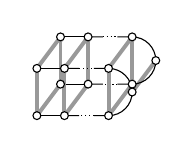
\begin{tikzpicture}
	\dynkin[name=1]{A}{IIIb}
	\node (a) at (-.3,-.4){};
	\dynkin[name=2,at=(a)]{A}{IIIb}
	\begin{scope}[on background layer]
		\foreach \i in {1,...,7}%
		{%
			\draw[/Dynkin diagram/fold style] 
				($(1 root \i)$) 
				-- 
				($(2 root \i)$);%
		}%
	\end{scope}
\end{tikzpicture}
\end{tcblisting}
\begin{tcblisting}{}
\pgfkeys{/Dynkin diagram,
edge length=.75cm,
edge/.style={draw=example-color,double=black,very thick}}
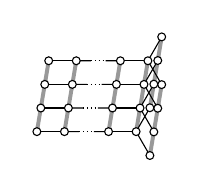
\begin{tikzpicture}
	\foreach \d in {1,...,4}
	{
		\node (current) at ($(\d*.05,\d*.3)$){};
		\dynkin[name=\d,at=(current)]{D}{oo.oooo}
	}
	\begin{scope}[on background layer]
		\foreach \i in {1,...,6}%
		{%
			\draw[/Dynkin diagram/fold style] ($(1 root \i)$) -- ($(2 root \i)$);%
			\draw[/Dynkin diagram/fold style] ($(2 root \i)$) -- ($(3 root \i)$);%
			\draw[/Dynkin diagram/fold style] ($(3 root \i)$) -- ($(4 root \i)$);%
		}%
	\end{scope}
\end{tikzpicture}
\end{tcblisting}

\section{Other examples}
\begin{filecontents*}{d44.tex}
\tikzset{/Dynkin diagram,edge length=1cm,fold radius=1cm}
\tikzset{/Dynkin diagram,label macro/.code={\alpha_{#1}},label macro*/.code={\beta_{#1}}}
\({}^1 D_4\) 4-ply tied straight:
\begin{dynkinDiagram}[ply=4]{D}[1]%
{****.*****.*****}
 \dynkinFold{0}{1}
 \dynkinFold{1}{13}
 \dynkinFold{13}{14}
\dynkinLabelRoots{0,...,14}
\dynkinLabelRoots*{0,...,14}
\end{dynkinDiagram}
\({}^1 D_4\) 4-ply tied bending:
\begin{dynkinDiagram}[ply=4]{D}[1]%
{****.*****.*****}
	\dynkinFold[bend right=65]{1}{13}
	\dynkinFold[bend right=65]{0}{14}
\dynkinLabelRoots{0,...,14}
\dynkinLabelRoots*{0,...,14}
\end{dynkinDiagram}
\end{filecontents*}
\begingroup\input{d44}\endgroup
\VerbatimInput{d44.tex}
Below we draw the Vogan diagrams of some affine Lie superalgebras \cite{Ransingh:2013,Ransingh:unpub}.
\begingroup
\tikzset{/Dynkin diagram,edge length=.35cm,fold radius=.3cm}
\NewDocumentCommand\labls{m}%
{%
	\ifcase#1%
		{1}\or%
		{1}\or%
		{2}\or%
		{2}\or%
		{2}\or%
		{2}\or%
		{2}\or%
		{1}\or%
		{1}\or%
		\else\typeout{What?}%
		\fi%
}%
\NewDocumentCommand\lablIt{m}%
{%
	\ifnum#1=0\relax%
		1%
	\else
		2%
	\fi%
}%
\begingroup
\tikzset{/Dynkin diagram,label macro/.code=\labls{#1},label,root radius=.06cm}
\tcbset{text width=10cm}
\RenewDocumentCommand\wdtA{}{2cm}
\NewDocumentEnvironment{Category}{m}%
{%
\begin{tcolorbox}[title={\(#1\)},breakable]{}
}%
{%
\end{tcolorbox}
}%

\begin{Category}{\mathfrak{sl}\left(2m|2n\right)^{(2)}}
\begin{tcblisting}{}
\begin{dynkinDiagram}[ply=2,label]{B}[1]{oo.oto.oo}
	\dynkinLabelRoot*{7}{1}
\end{dynkinDiagram}
\end{tcblisting}
\begin{tcblisting}{}
\dynkin[label]{B}[1]{oo.oto.oo}
\end{tcblisting}
\begin{tcblisting}{}
\dynkin[ply=2,label]{B}[1]{oo.Oto.Oo}
\end{tcblisting}
\begin{tcblisting}{}
\dynkin[label]{B}[1]{oo.Oto.Oo}
\end{tcblisting}
\begin{tcblisting}{}
\dynkin[label]{D}[1]{oo.oto.ooo}
\end{tcblisting}
\begin{tcblisting}{}
\dynkin[label]{D}[1]{oO.otO.ooo}
\end{tcblisting}
\begin{tcblisting}{}
\dynkin[label,fold]{D}[1]{oo.oto.ooo}
\end{tcblisting}
\end{Category}

\begin{Category}{\mathfrak{sl}\left(2m+1|2n\right)^2}
\begin{tcblisting}{}
\dynkin[label]{B}[1]{oo.oto.oo}
\end{tcblisting}
\begin{tcblisting}{}
\dynkin[label]{B}[1]{oO.oto.oO}
\end{tcblisting}
\begin{tcblisting}{}
\dynkin[label,fold]{B}[1]{oo.oto.oo}
\end{tcblisting}
\end{Category}

\begin{Category}{\mathfrak{sl}\left(2m+1|2n+1\right)^2}
\begin{tcblisting}{}
\dynkin[label]{D}[2]{o.oto.oo}
\end{tcblisting}
\begin{tcblisting}{}
\dynkin[label]{D}[2]{o.OtO.oo}
\end{tcblisting}
\end{Category}

\begin{Category}{\mathfrak{sl}\left(2|2n+1\right)^{(2)}}
\begin{tcblisting}{}
\dynkin[ply=2,label,double edges]{B}[1]{oo.Oto.Oo}
\end{tcblisting}
\begin{tcblisting}{}
\dynkin[ply=2,label,double fold]{B}[1]{oo.Oto.Oo}
\end{tcblisting}
\begin{tcblisting}{}
\dynkin[ply=2,label,double edges]{B}[1]{oo.OtO.oo}
\end{tcblisting}
\begin{tcblisting}{}
\dynkin[ply=2,label,double fold]{B}[1]{oo.OtO.oo}
\end{tcblisting}
\end{Category}

\begin{Category}{\mathfrak{sl}\left(2|2n\right)^{(2)}}
\begin{tcblisting}{}
\dynkin[ply=2,label,double edges]{D}[1]{oo.oto.ooo}
\end{tcblisting}
\begin{tcblisting}{}
\dynkin[ply=2,label,double fold left]{D}[1]{oo.oto.ooo}
\end{tcblisting}
\end{Category}

\begin{Category}{\mathfrak{osp}\left(2m|2n\right)^{(2)}}
\begin{tcblisting}{}
\dynkin[label,label macro/.code={1}]{D}[2]{o.oto.oo}
\end{tcblisting}
\begin{tcblisting}{}
\dynkin[label,label macro/.code={1}]{D}[2]{o.Oto.Oo}
\end{tcblisting}
\end{Category}

\begin{Category}{\mathfrak{osp}\left(2|2n\right)^{(2)}}
\begin{tcblisting}{}
\dynkin[label,label macro/.code=\lablIt{#1},
	affine mark=*]
	{D}[2]{o.o.o.o*}
\end{tcblisting}
\begin{tcblisting}{}
\dynkin[label,label macro/.code=\lablIt{#1},
	affine mark=*]
	{D}[2]{o.O.o.o*}
\end{tcblisting}
\end{Category}

\begin{Category}{\mathfrak{sl}\left(1|2n+1\right)^{4}}
\begin{tcblisting}{}
\dynkin[label,label macro/.code={1}]{D}[2]{o.o.o.o*}
\end{tcblisting}
\begin{tcblisting}{}
\dynkin[label,label macro/.code={1}]{D}[2]{o.o.O.o*}
\end{tcblisting}
\end{Category}


\begin{Category}{A^1}
\begin{tcblisting}{}
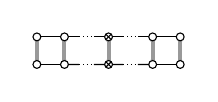
\begin{tikzpicture}
	\dynkin[name=upper]{A}{oo.t.oo}
	\node (Dynkin current) at (upper root 1){};
	\dynkinSouth
	\dynkin[at=(Dynkin current),name=lower]{A}{oo.t.oo}
	\begin{scope}[on background layer]
	\foreach \i in {1,...,5}{
		\draw[/Dynkin diagram/fold style] 
			($(upper root \i)$) -- ($(lower root \i)$);
	}
	\end{scope}
\end{tikzpicture}
\end{tcblisting}
\begin{tcblisting}{}
\dynkin[fold]{A}[1]{oo.t.ooooo.t.oo}
\end{tcblisting}
\begin{tcblisting}{}
\dynkin[fold,affine mark=t]{A}[1]{oo.o.ootoo.o.oo}
\end{tcblisting}
\begin{tcblisting}{}
\dynkin[affine mark=t]{A}[1]{o*.t.*o}
\end{tcblisting}
\end{Category}

\begin{Category}{B^1}
\begin{tcblisting}{}
\dynkin[affine mark=*]{A}[2]{o.oto.o*}
\end{tcblisting}
\begin{tcblisting}{}
\dynkin[affine mark=*]{A}[2]{o.oto.o*}
\end{tcblisting}
\begin{tcblisting}{}
\dynkin[affine mark=*]{A}[2]{o.ooo.oo}
\end{tcblisting}
\begin{tcblisting}{}
\dynkin[odd]{A}[2]{oo.*to.*o}
\end{tcblisting}
\begin{tcblisting}{}
\dynkin[odd,fold]{A}[2]{oo.oto.oo}
\end{tcblisting}
\begin{tcblisting}{}
\dynkin[odd,fold]{A}[2]{o*.oto.o*}
\end{tcblisting}
\end{Category}

\begin{Category}{D^1}
\begin{tcblisting}{}
\dynkin{D}{otoo}
\end{tcblisting}
\begin{tcblisting}{}
\dynkin{D}{ot*o}
\end{tcblisting}
\begin{tcblisting}{}
\dynkin[fold]{D}{otoo}
\end{tcblisting}
\end{Category}

\begin{Category}{C^1}
\begin{tcblisting}{}
\dynkin[double edges,fold,affine mark=t,odd]{A}[2]{to.o*}
\end{tcblisting}
\begin{tcblisting}{}
\dynkin[double edges,fold,affine mark=t,odd]{A}[2]{t*.oo}
\end{tcblisting}
\end{Category}

\begin{Category}{F^1}
\begin{tcblisting}{}
\begin{dynkinDiagram}{A}{oto*}%
	\dynkinQuadrupleEdge{1}{2}%
	\dynkinTripleEdge{4}{3}%
\end{dynkinDiagram}%
\end{tcblisting}
\begin{tcblisting}{}
\begin{dynkinDiagram}{A}{*too}%
	\dynkinQuadrupleEdge{1}{2}%
	\dynkinTripleEdge{4}{3}%
\end{dynkinDiagram}%
\end{tcblisting}
\end{Category}

\begin{Category}{G^1}
\begin{tcblisting}{}
\begin{dynkinDiagram}{A}{ot*oo}%
	\dynkinQuadrupleEdge{1}{2}%
	\dynkinDefiniteDoubleEdge{4}{3}%
\end{dynkinDiagram}%
\end{tcblisting}
\begin{tcblisting}{}
\begin{dynkinDiagram}{A}{oto*o}%
	\dynkinQuadrupleEdge{1}{2}%
	\dynkinDefiniteDoubleEdge{4}{3}%
\end{dynkinDiagram}%
\end{tcblisting}
\begin{tcblisting}{}
\begin{dynkinDiagram}{A}{*too*}%
	\dynkinQuadrupleEdge{1}{2}%
	\dynkinDefiniteDoubleEdge{4}{3}%
\end{dynkinDiagram}%
\end{tcblisting}
\begin{tcblisting}{}
\begin{dynkinDiagram}{A}{*tooo}%
	\dynkinQuadrupleEdge{1}{2}%
	\dynkinDefiniteDoubleEdge{4}{3}%
\end{dynkinDiagram}%
\end{tcblisting}
\end{Category}
\endgroup


\begin{filecontents*}{simple-lie-algebras.tex}
\NewDocumentEnvironment{bunch}{}%
{\renewcommand*{\arraystretch}{1}\begin{array}{@{}ll@{}}\\ \midrule}{\\ \midrule\end{array}}
\small
\NewDocumentCommand\nct{mm}{\newcolumntype{#1}{>{\columncolor[gray]{.9}}>{$}m{#2cm}<{$}}}
\nct{G}{.3}\nct{D}{2.1}\nct{W}{3}\nct{R}{3.7}\nct{S}{3}
\NewDocumentCommand\LieG{}{\mathfrak{g}}
\NewDocumentCommand\W{om}{\ensuremath{\mathbb{Z}^{#2}\IfValueT{#1}{/\left<#1\right>}}}
\renewcommand*{\arraystretch}{1.5}
\NewDocumentCommand\quo{}{\text{quotient of } E_8}
\begin{longtable}{@{}GDWRS@{}}
\LieG&\text{Diagram}&\text{Weights}&\text{Roots}&\text{Simple roots}\\ \midrule\endfirsthead
\LieG&\text{Diagram}&\text{Weights}&\text{Roots}&\text{Simple roots}\\ \midrule\endhead
A_n&\dynkin{A}{}&\frac{1}{r+1}\W[\sum e_j]{n+1}&e_i-e_j&e_i-e_{i+1}\\
B_n&\dynkin{B}{}&\frac{1}{2}\W{n}& \pm e_i, \pm e_i \pm e_j, i\ne j&e_i-e_{i+1}, e_n\\
C_n&\dynkin{C}{}&\W{n}& \pm 2 e_i, \pm e_i \pm e_j, i\ne j&e_i-e_{i+1}, 2e_n\\
D_n&\dynkin{D}{}&\frac{1}{2}\W{n}& \pm e_i \pm e_j, i\ne j &
\begin{bunch}e_i-e_{i+1},&i\le n-1\\e_{n-1}+e_n\end{bunch}\\
E_8&\dynkin{E}{8}&\frac{1}{2}\W{8}&
\begin{bunch}\pm2e_i\pm2e_j,&i\ne j,\\ \sum_i(-1)^{m_i}e_i,&\sum m_i \text{ even}\end{bunch}&
\begin{bunch}
2e_1-2e_2,\\2e_2-2e_3,\\2e_3-2e_4,\\2e_4-2e_5,\\2e_5-2e_6,\\2e_6+2e_7,\\
-\sum e_j,\\2e_6-2e_7
\end{bunch}\\
E_7&\dynkin{E}{7}&\frac{1}{2}\W[e_1-e_2]{8}&\quo&\quo\\
E_6&\dynkin{E}{6}&\frac{1}{3}\W[e_1-e_2,e_2-e_3]{8}&\quo&\quo\\
F_4& \dynkin{F}{4}&\W{4}&
\begin{bunch}\pm 2e_i,\\ \pm 2e_i \pm 2e_j, \quad i \ne j,\\ \pm e_1 \pm e_2 \pm e_3 \pm e_4
\end{bunch}&
\begin{bunch}2e_2-2e_3,\\2e_3-2e_4,\\2e_4,\\e_1-e_2-e_3-e_4\end{bunch}\\
G_2&\dynkin{G}{2}&\W[\sum e_j]{3}&
\begin{bunch}
\pm(1,-1,0),\\ \pm(-1,0,1),\\ \pm(0,-1,1),\\ \pm(2,-1,-1),\\ \pm(1,-2,1),\\ \pm(-1,-1,2)
\end{bunch}&
\begin{bunch}(-1,0,1),\\(2,-1,-1)\end{bunch}
\end{longtable}
\end{filecontents*}
\begingroup
\input{simple-lie-algebras.tex}
\endgroup
\VerbatimInput{simple-lie-algebras.tex}

\begin{filecontents*}{borovoi.tex}
\tikzset{big arrow/.style={
	-Stealth,line cap=round,line width=1mm,
	shorten <=1mm,shorten >=1mm}}
\newcommand\catholic[2]{\draw[big arrow,green!25!white] 
(root #1) to (root #2);}
\newcommand\protestant[2]{
\begin{scope}[transparency group, opacity=.25]
\draw[big arrow,orange] (root #1) to (root #2);
\end{scope}}
\begin{dynkinDiagram}[edge length=1.2cm,
indefinite edge/.style={thick,loosely dotted},
labels*={0,1,2,3,\ell-3,\ell-2,\ell-1,\ell}]{D}[1]{}
\catholic{0}{6}\catholic{1}{7}
\protestant{7}{0}\protestant{6}{1}
\end{dynkinDiagram}
\end{filecontents*}
\begingroup
\begin{center}
\input{borovoi.tex}
\end{center}
\endgroup
\VerbatimInput{borovoi.tex}
\newpage


\section{Syntax}
The syntax is \verb!\dynkin[<options>]{<letter>}[<twisted rank>]{<rank>}! where \verb!<letter>! is \verb!A!, \verb!B!, \verb!C!, \verb!D!, \verb!E!, \verb!F! or \verb!G!, the family of root system for the Dynkin diagram, \verb!<twisted rank>! is \verb!0!, \verb!1!, \verb!2!, \verb!3! (default is \verb!0!) representing:
\[
\renewcommand*{\arraystretch}{1}
\begin{array}{rp{8cm}}
0 & finite root system \\ \hline
1 & affine extended root system, i.e.  of type \({}^{(1)}\) \\
2 & affine twisted root system of type \({}^{(2)}\) \\
3 & affine twisted root system of type \({}^{(3)}\) \\
\end{array}
\]
and \verb!<rank>! is 
\begin{enumerate}
\item
an integer representing the rank or 
\item
blank to represent an indefinite rank or
\item
the name of a Satake diagram as in section~\ref{section:Satake}.
\end{enumerate}
The environment syntax is \verb!\begin{dynkinDiagram}! followed by the same parameters as \verb!\dynkin!, then various Dynkin diagram and \TikZ{} commands, and then \verb!\end{dynkinDiagram}!.

\section{Options}
\newcommand*{\typ}[1]{\(\left<\texttt{#1}\right>\)}
\newcommand*{\optionLabel}[3]{%%
\multicolumn{2}{l}{\(\texttt{#1}=\texttt{#2}\),} \\
\multicolumn{2}{l}{\(\textrm{default}: \texttt{#3}\)} \\
}%%
\renewcommand*{\arraystretch}{1}
\par\noindent%
\begin{longtable}{p{1cm}p{10cm}}
\endfirsthead
\caption{\dots continued}\\
\endhead
\multicolumn{2}{c}{continued \dots}\\
\endfoot
\endlastfoot
\optionLabel{text/.style}{\typ{TikZ style data}}{scale=.7}
& Style for any labels on the roots. \\
\optionLabel{name}{\typ{string}}{anonymous}
& A name for the Dynkin diagram, with \texttt{anonymous} treated as a blank; see section~\ref{section:name}. \\
\optionLabel{parabolic}{\typ{integer}}{0} 
& A parabolic subgroup with specified integer, where the integer
is computed as \(n=\sum 2^{i-1} a_i\), \(a_i=0\) or \(1\), to say that root \(i\) is crossed, i.e. a noncompact root. \\
\optionLabel{root radius}{\typ{number}cm}{.05cm}
&      size of the dots and of the crosses in the Dynkin diagram \\
\optionLabel{edge length}{\typ{number}cm}{.35cm}
&      distance between nodes in the Dynkin diagram \\
\optionLabel{edge/.style}{TikZ style data}{thin}
&      style of edges in the Dynkin diagram \\
\optionLabel{mark}{\typ{o,O,t,x,X,*}}{*}
&      default root mark \\
\optionLabel{affine mark}{o,O,t,x,X,*}{*}
&      default root mark for root zero in an affine Dynkin diagram \\
\optionLabel{label}{true or false}{false}
& whether to label the roots according to the current labelling scheme. \\
\optionLabel{label macro}{\typ{1-parameter \TeX{} macro}}{\texttt{\#1}}
& the current labelling scheme for roots. \\
\optionLabel{label macro*}{\typ{1-parameter \TeX{} macro}}{\texttt{\#1}}
& the current labelling scheme for alternate roots. \\
\optionLabel{make indefinite edge}{\typ{edge pair \(i\)-\(j\) or list of such}}{\{\}}
& edge pair or list of edge pairs to treat as having indefinitely many roots on them. \\
\optionLabel{indefinite edge ratio}{\typ{float}}{1.6}
& ratio of indefinite edge lengths to other edge lengths. \\
\optionLabel{indefinite edge/.style}{\typ{TikZ style data}}{draw=black,fill=white,thin,densely dotted}
& style of the dotted or dashed middle third of each indefinite edge. \\
\optionLabel{backwards}{\typ{true or false}}{false}
& whether to reverse right to left. \\
\optionLabel{upside down}{\typ{true or false}}{false}
& whether to reverse up to down. \\
\optionLabel{arrows}{\typ{true or false}}{true}
& whether to draw the arrows that arise along the edges. \\
\optionLabel{reverse arrows}{\typ{true or false}}{true}
& whether to reverse the direction of the arrows that arise along the edges. \\
\optionLabel{fold}{\typ{true or false}}{true}
& whether, when drawing Dynkin diagrams, to draw them 2-ply. \\
\optionLabel{ply}{\typ{0,1,2,3,4}}{0}
& how many roots get folded together, at most. \\
\optionLabel{fold left}{\typ{true or false}}{true}
& whether to fold the roots on the left side of a Dynkin diagram. \\
\optionLabel{fold right}{\typ{true or false}}{true}
& whether to fold the roots on the right side of a Dynkin diagram. \\
\optionLabel{fold radius}{\typ{length}}{.3cm}
& the radius of circular arcs used in curved edges of folded Dynkin diagrams. \\
\optionLabel{fold style}{\typ{TikZ style data}}{draw=black!40,fill=none,line width=radius}
& when drawing folded diagrams, style for the fold indicators. \\
\optionLabel{*/.style}{\typ{TikZ style data}}{draw=black,fill=black}
& style for roots like \dynkin{A}{*} \\
\optionLabel{o/.style}{\typ{TikZ style data}}{draw=black,fill=black}
& style for roots like \dynkin{A}{o}  \\
\optionLabel{O/.style}{\typ{TikZ style data}}{draw=black,fill=black}
& style for roots like \dynkin{A}{O}  \\
\optionLabel{t/.style}{\typ{TikZ style data}}{draw=black,fill=black}
& style for roots like \dynkin{A}{t} \\
\optionLabel{x/.style}{\typ{TikZ style data}}{draw=black,line cap=round}
& style for roots like \dynkin{A}{x}  \\
\optionLabel{X/.style}{\typ{TikZ style data}}{draw=black,thick,line cap=round}
& style for roots like \dynkin{A}{X} \\
\optionLabel{fold left style/.style}{\typ{TikZ style data}}{}
& style to override the \texttt{fold} style when folding roots together on the left half of a Dynkin diagram \\
\optionLabel{fold right style/.style}{\typ{TikZ style data}}{}
& style to override the \texttt{fold} style when folding roots together on the right half of a Dynkin diagram \\
\optionLabel{double edges}{\typ{}}{not set}
& set to override the \texttt{fold} style when folding roots together in a Dynkin diagram, so that the foldings
are indicated with double edges (like those of an \(F_4\) Dynkin diagram without arrows). \\
\optionLabel{double fold}{\typ{}}{not set}
& set to override the \texttt{fold} style when folding roots together in a Dynkin diagram, so that the foldings
are indicated with double edges (like those of an \(F_4\) Dynkin diagram without arrows), but filled in solidly. \\
\optionLabel{double left}{\typ{}}{not set}
& set to override the \texttt{fold} style when folding roots together at the left side of a Dynkin diagram, so that the foldings are indicated with double edges (like those of an \(F_4\) Dynkin diagram without arrows). \\
\optionLabel{double fold left}{\typ{}}{not set}
& set to override the \texttt{fold} style when folding roots together  at the left side of a Dynkin diagram, so that the foldings are indicated with double edges (like those of an \(F_4\) Dynkin diagram without arrows), but filled in solidly. \\
\optionLabel{double right}{\typ{}}{not set}
& set to override the \texttt{fold} style when folding roots together at the right side of a Dynkin diagram, so that the foldings are indicated with double edges (like those of an \(F_4\) Dynkin diagram without arrows). \\
\optionLabel{double fold right}{\typ{}}{not set}
& set to override the \texttt{fold} style when folding roots together  at the right side of a Dynkin diagram, so that the foldings are indicated with double edges (like those of an \(F_4\) Dynkin diagram without arrows), but filled in solidly.
\\
\optionLabel{arrow color}{\typ{}}{black}
& set to override the default color for the arrows in nonsimply laced Dynkin diagrams. \\
\optionLabel{Coxeter}{\typ{true or false}}{false}
& whether to draw a Coxeter diagram, rather than a Dynkin diagram. \\
\optionLabel{ordering}{\typ{Adams, Bourbaki, Carter, Dynkin, Kac}}{Bourbaki}
& which ordering of the roots to use in exceptional root systems as in section~\ref{section:order}. \\
\end{longtable}
\par\noindent{}All other options are passed to TikZ.

\section{Changes in the latest version}\label{section:changes}
\begin{center}
\begin{tabular}{@{}>{\ttfamily}r>{\ttfamily}l>{\ttfamily}l@{}}
\textrm{was} & \textrm{is} & \textrm{or as a global option} \\ \midrule
edgeLength&edge length&edge-length\\
radius&root radius&root-radius\\
affineMark&affine mark&affine-mark\\
labelMacro&label macro&label-macro\\
makeIndefiniteEdge&make indefinite edge&make-indefinite-edge\\
indefiniteEdgeRatio&indefinite edge ratio&indefinite-edge-ratio\\
indefiniteEdge&indefinite edge&indefinite-edge\\
reverseArrows&reverse arrows&reverse-arrows\\
foldLeft&fold left&fold-left\\
foldRight&fold right&fold-right\\
foldradius&fold radius&fold-radius\\
foldStyle&fold style&fold-style\\
leftFoldStyle&fold left style&fold-left-style\\
rightFoldStyle&fold right style&fold-right-style\\
doubleEdges&double edges&double-edges\\
doubleFold&double fold&double-fold\\
doubleLeft&double left&double-left\\
doubleLeftFold&double fold left&double-fold-left\\
doubleRight&double right&double-right\\
doubleRightFold&double fold right&double-fold-right\\
arrowColor&arrow color&arrow-color\\
\end{tabular}
\end{center}


\nocite{*}
\bibliographystyle{amsplain}
\bibliography{dynkin-diagrams}
\end{document}
